\documentclass[11pt]{article}
\usepackage[english]{babel}  % Croatian typographical rules and hyphenation patterns
\usepackage{ae,aecompl}     	% Type 1 fonts, similar to Computer Modern

\usepackage{microtype}				% Improves spacing

\usepackage{booktabs}					% Nice looking tables
\usepackage{enumerate}				% Additional options for listing of items in enumerate environment
\usepackage{algorithm2e}			% Writing pseudo-code
\usepackage{todonotes}				% Adding todo items
\usepackage{dirtree}					% Simple display of directory tree
\usepackage{hyperref}

\usepackage{graphicx}
\usepackage{subfig}
\usepackage{caption}
\usepackage{listings}

\hypersetup{
    colorlinks=true,
    linkcolor=blue,
    filecolor=magenta,
    urlcolor=cyan,
}
\urlstyle{same}
\usepackage{graphics}

\graphicspath{ {./images/} }

\title{
	\Large Josip Juraj Strossmayer University of Osijek \\
	Faculty of Electrical Engineering, Computer Science and Information
	 Technologies\\
	\vspace{4cm}
	\Large Course: Linux in Embedded Systems \\
	\vspace{4cm}
	\Large \textbf{Laboratory exercise 2: Getting familiar with Raspberry Pi
		3.\\
		Building Linux for Raspberry Pi 3}
	}
\date{}
\begin{document}
\maketitle
\thispagestyle{empty}
\newpage

\section{Introduction}
The Raspberry Pi computer was launched in early 2012 and launched a revolution
 in the field of computer related education and hobbies. This computer has
 become extremely popular because of its price (around \$35) and small
 dimensions (8.6cm x 5.4cm x 1.7cm). Although the Raspberry Pi is a
 general-purpose computer, it has the ability to connect different equipment
 (e.g. different sensors and actuators) so it is used in many hobby projects in
 different embedded computer systems and IoT (Internet of Things) areas, and
 increasingly in various commercial projects. The main part of this computer
 represents SoC (System On a Chip) with a different periphery like
 RAM, HDMI output, Ethernet port, etc. Also on the board there are General
 Purpose Input Output (GPIO) pins that enable connecting different equipment.

\section{Raspberry Pi Models}
To date, several generations of Raspberry Pi computers have been released.
 All in common with Broadcom SoC consisting integrated ARM processor (CPU)
 and a built-in GPU. The processor clock speed is moving from 700 MHz to 1.4 GHz
 for Pi 3B+ or 1.5 GHz for Pi 4. The amount of memory (RAM) ranges from 256 MB
 to 1 GB or even 4 GB code on strongest model of the latest Pi 4. Secure Digital
 (SD) cards are used for storage of the operating system and programs.
 There are up to four USB ports on the board. HDMI is used for video output.
 Using GPIO pins standard protocols such as I\textsuperscript{2}C are supported.
 All B models have Ethernet connection, while the Pi 3 and Pi Zero W have Wi-Fi
 802.11n and Bluetooth.
\newline
\newline
Smaller-sized Raspberry Pi Zero with reduced set of input-output units and
 general purpose input and output units (GPIO) was released to market in 2015
 with a price tag of \$5. In 2017, the Raspberry Pi Zero W with added Wi-Fi and
 Bluetooth capabilities was released.
The Raspberry Pi 3 Model B was released in 2016 with 1.2 GHz 64-bit quad-core
 processor and built-in 802.11n Wi-Fi and Bluetooth capabilities. In 2018, the
 Raspberry Pi 3 Model B+ with 1.4 GHz processor and gigabit Ethernet
network (by actual tests it reaches a speed of 300 Mbit/s because it shares a
USB 2.0 bus) was released.
 It comes with dual-band 802.11ac 2.4/5 Ghz Wi-Fi wireless networking.
\begin{figure}[h!]
\centering
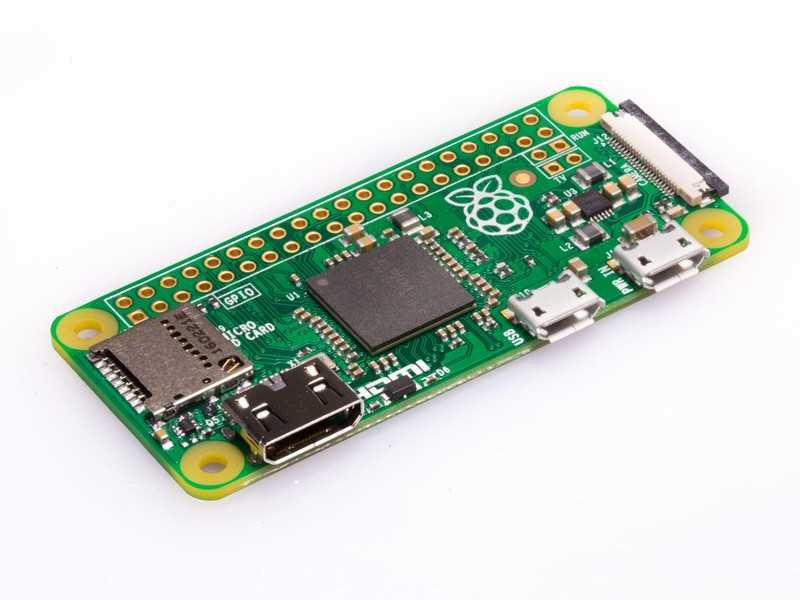
\includegraphics[width=0.8\textwidth]{rpi-zero.jpg}
\captionsetup{justification=centering}
\caption{Raspberry Pi Zero}
\end{figure}
The latest Raspberry Pi Model 4 B was released in 2019. It has 1.5 GHz
 quad-core ARM Cortex-A72 processor, 802.11ac supported Wi-Fi,
 Bluetooth 5 support, fully supported Gigabit Ethernet, two USB 2.0 ports, two
 USB 3.0 ports and a support for 4K video resolution.
\newline
\newline
On laboratory exercises \textbf{Raspberry Pi 3 B} will be used.
\newline
\newline
Technical specifications of Raspberry Pi 3 B: \\
\textbf{SoC}: Broadcom BCM2837 \\
\textbf{CPU}: quad-core ARM Cortex-A53, 1.2GHz \\
\textbf{GPU}: Broadcom VideoCore IV \\
\textbf{RAM}: 1GB LPDDR2 (900 MHz) \\
\textbf{Network}: 10/100 Ethernet, 2.4GHz 802.11n wireless \\
\textbf{Bluetooth}: Bluetooth 4.1 Classic, Bluetooth Low Energy \\
\textbf{Storage}: MicroSD \\
\textbf{GPIO}: 40-pin header, populated \\
\textbf{I/O}: $4\times USB 2.0$, HDMI, 3.5mm analogni priključak,
 Ethernet, \textit{Camera Serial Interface} (CSI), \textit{Display Serial
 Interface} (DSI)

 \begin{figure}[h!]
\centering
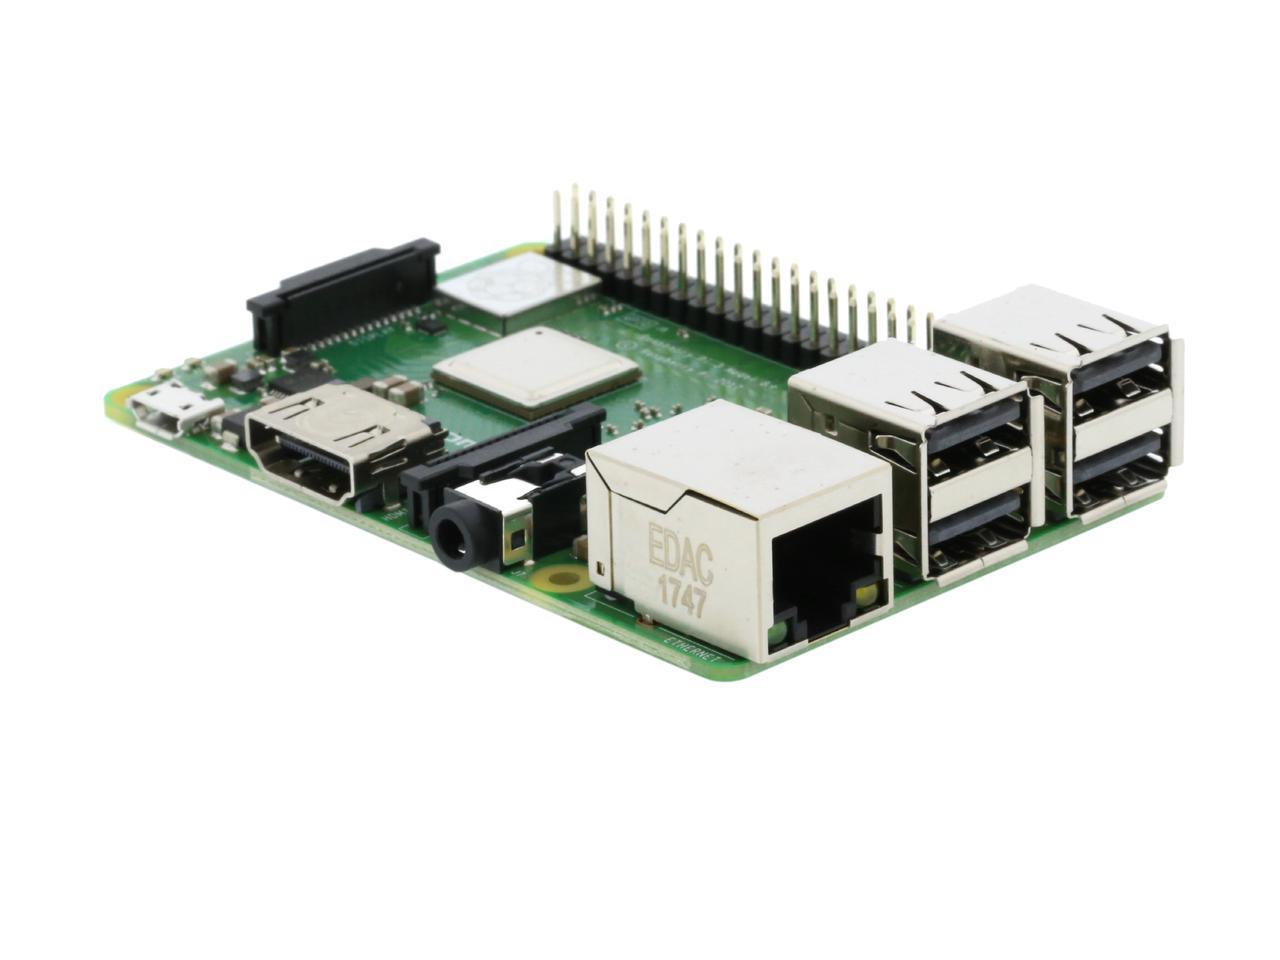
\includegraphics[width=0.8\textwidth]{rpi-3-b-plus.jpg}
\captionsetup{justification=centering}
\caption{Raspberry Pi 3 B+}
\end{figure}
\begin{figure}[h!]
\centering
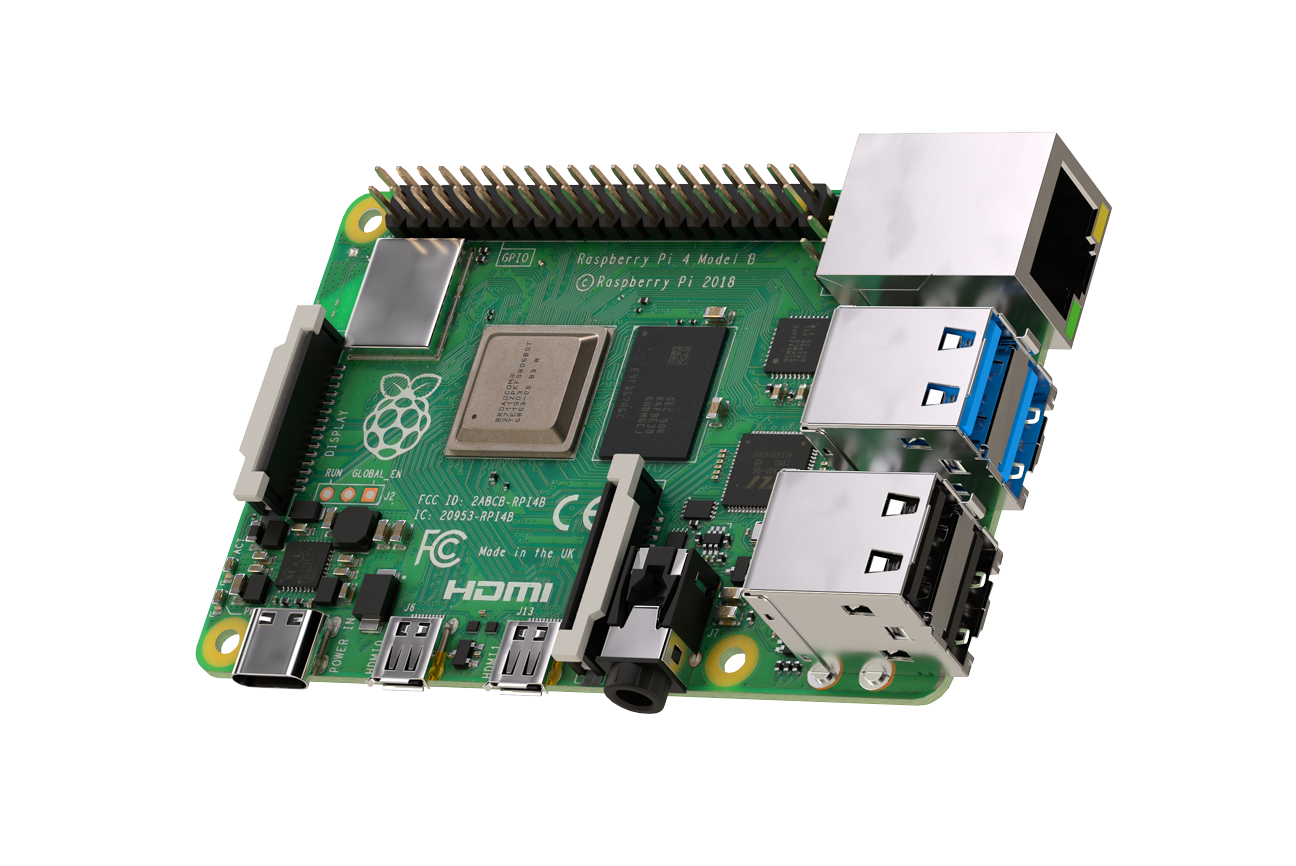
\includegraphics[width=0.8\textwidth]{rpi-4.png}
\captionsetup{justification=centering}
\caption{Raspberry Pi 4 B}
\end{figure}

\begin{figure}
\centering
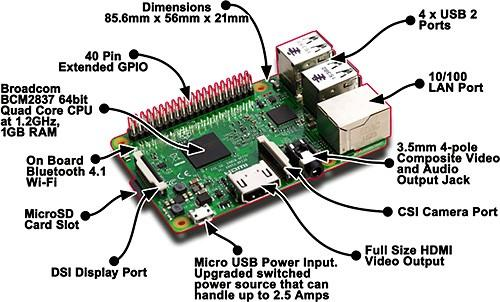
\includegraphics[width=0.8\textwidth]{rpi-3-details.jpg}
\captionsetup{justification=centering}
\caption{Raspberry Pi 3 details}
\end{figure}
\begin{figure}[h!]
	\centering
	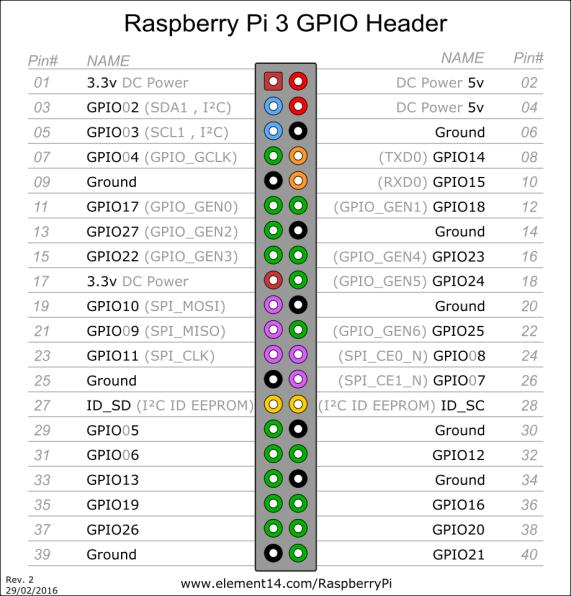
\includegraphics[width=0.8\textwidth]{rpi-3-pins.jpg}
	\captionsetup{justification=centering}
	\caption{Raspberry Pi 3 GPIO}
	\label{fig:rpi-gpio}
\end{figure}

\clearpage
\section{Additional equipment}
Apart from the Raspberry Pi itself, various accessories are required
depending on the application:
\begin{enumerate}
	\item power supply 5V 2A, USB micro connector
	\item micro SD memory card, capacity min. 4GB Class A
	\item USB converter to serial cable communication (UART)
	\item USB converter to Ethernet and Ethernet cable
	\item additional driver development devices.
\end{enumerate}

\begin{figure}
    \centering
    \subfloat[Power supply]{{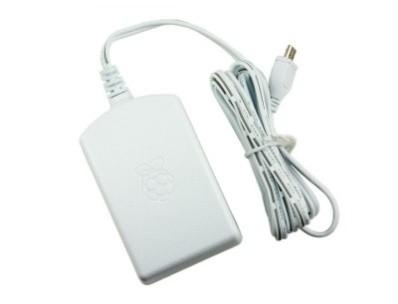
\includegraphics[width=4cm]{rpi-charger.jpg}}}%
    \subfloat[SD card]{{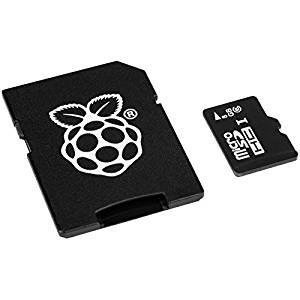
\includegraphics[width=4cm]{rpi-sdcard.jpg}}}%
    \subfloat[USB UART]{{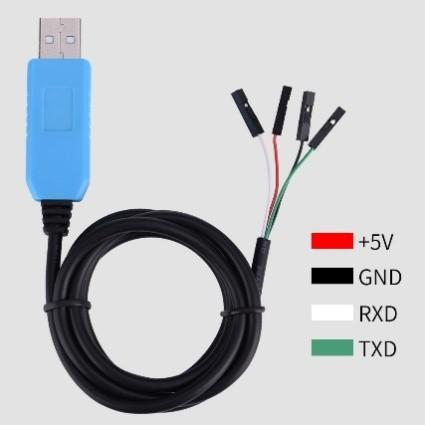
\includegraphics[width=4cm]{rpi-uart.jpg}}}%
    \qquad
    \subfloat[USB Ethernet]{{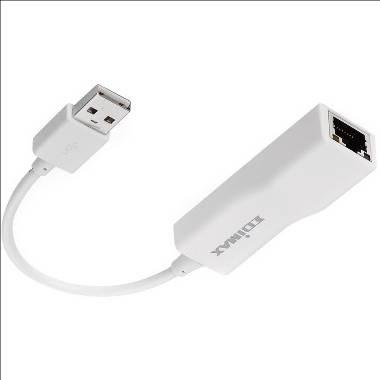
\includegraphics[width=4cm]{rpi-ethernet.jpg}}}%
    \subfloat[Nunchuk]{{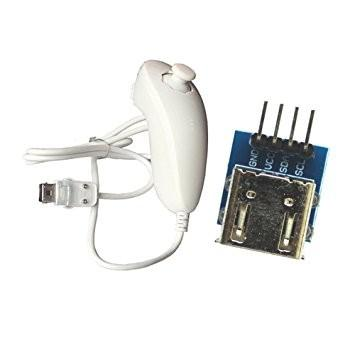
\includegraphics[width=4cm]{rpi-nunchuk.jpg}}}%
    \subfloat[Case]{{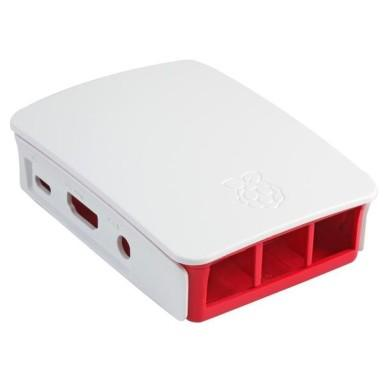
\includegraphics[width=4cm]{rpi-case.jpg}}}%
    \caption{Raspberry Pi accessories}%
    \label{fig:equipment1}%
\end{figure}

\section{Initial setup}
If you don't have your \texttt{embedded\_linux} repository on your development
 computer, first clone it with the appropriate command from your Gitlab account
 into your \textit{home} directory. Position yourself in the\\
 \texttt{/home/rtrk/embedded\_linux} directory. Then pull the possible changes
 from the source repository using the command:
\begin{lstlisting}[language=bash]
git remote add upstream
	https://gitlab.com/rgrbic/embedded_linux
git fetch upstream
git merge upstream/master
\end{lstlisting}
Install additional tools using command:
Instalirajte potrebne alate na razvojno računalo:
\begin{lstlisting}[language=bash]
sudo apt-get install gcc-arm-linux-gnueabihf
\end{lstlisting}

\end{document}
